\documentclass[12pt]{article}
\usepackage{amsmath}
\usepackage{askmaps}
\usepackage{graphicx}
\usepackage{wrapfig}
\usepackage{booktabs}
\usepackage[letterpaper, margin=1in]{geometry}
\usepackage{fancyhdr}
\usepackage [autostyle, english = american]{csquotes}
\MakeOuterQuote{"}
\renewcommand{\baselinestretch}{1.0}
\newcommand{\twoobjects}[2]{%
  \leavevmode\vbox{\hbox{#1}\nointerlineskip\hbox{#2}}%
}
\title{Lab 4 \\ Verilog HDL}
\author{Qadis Chaudhry}
\date{April 9, 2021}
\begin{document}
\maketitle
    \section*{Half Adder}
    \begin{figure}[h]
        \centering
        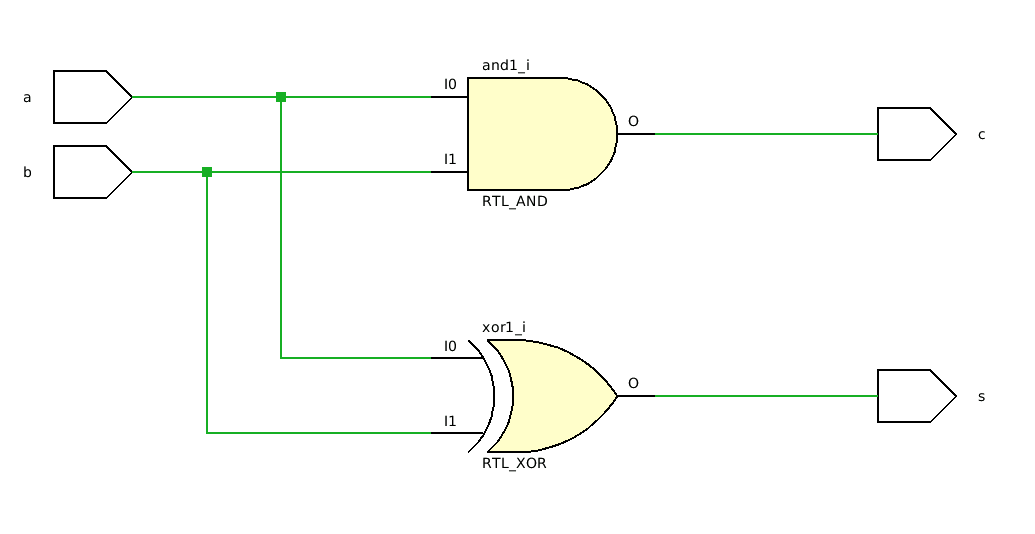
\includegraphics[width=0.7\textwidth]{Half Adder Schematic.png}
        \caption{Half Adder Schematic}
        \label{fig:Half-Adder-Schematic}
    \end{figure}
    \par The function of a half-adder is to provide the sum of two digits along
    with the carry out of their addition, if one happens to exist. It can be
    seen by this schematic, that the way this is achieved is by using an XOR
    gate and an AND gate where both the inputs serve as inputs to each of the
    gates. The XOR gate is used in the summation of the numbers while the AND
    gate, in the formation of the carry out. This function can be proven using a
    truth table where the inputs are the bits $A$ and $B$ and the outputs are
    the sum of the bits as well as the carry out of the summation.
    \begin{table}[h]
        \centering
        \begin{tabular}{cc|cc}
            \toprule
            $A$ & $B$ & $Sum$ & $C_{out}$ \\
            \midrule
            0 & 0 & 0 & 0 \\
            0 & 1 & 1 & 0 \\
            1 & 0 & 0 & 0 \\
            1 & 1 & 1 & 1 \\
            \bottomrule
        \end{tabular}
    \end{table}
    \par In this case, simply through the observation of the truth table can the
    functions for the two output variables can be deduced. For the Sum, the
    output of the table is recognizable as being the pattern of an XOR gate, and
    with that, the expression of the sum can be written as, $A \oplus B$. The
    function for $C_{out}$ is also evident as it is seen that $C_{out}$ is only
    equal to 1 when both $A$ and $B$ are equal to 1. This is the operation of
    the AND gate therefore, $C_{out}$ is equal to $AB$, completing the
    construction of the half adder.
    \par In order to implement this within Verilog, the two gates can be created
    and given the inputs $A$ and $B$, and the outputs can be specified as the
    sum and the carry out. These outputs will be coupled with their appropriate
    gates and form the half adder.
    \begin{figure}[h]
        \centering
        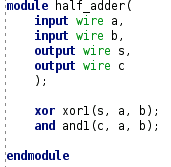
\includegraphics[width=0.3\textwidth]{Half Adder Code.png}
        \caption{Half Adder Code}
        \label{fig:Half-Adder-Code}
    \end{figure}
    \par Above is the code for the implementation of the half adder with the use
    of the Verilog HDL. The inputs are specified as wires with $a$ and $b$ being
    the inputs and $s$ and $c$ being the outputs, half sum and carry out,
    respectively. The module is named "half\_adder" and there are two functions
    present, "xor" and "and." The function "xor" denotes an XOR gate in the
    language and it can be seen that it is named "xor1." Further, it gives the
    output $s$, denoted by the first input of the function, and taking the
    inputs $a$ and $b$. The case is the same with the "and" function, named
    "and1," gives the output $c$, and takes the inputs $a$ and $b$.
    \section*{Full Adder}
    \begin{figure}[h]
        \centering
        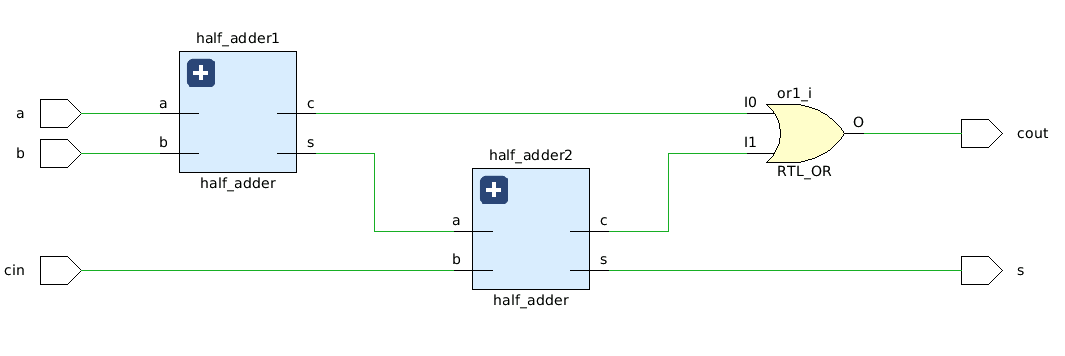
\includegraphics[width=0.8\textwidth]{Full Adder Schematic.png}
        \caption{Full Adder Schematic}
        \label{fig:Full-Adder-Schematic}
    \end{figure}
    \par This figure shows the schematic of a full adder as it is implemented
    using two half adders and one OR gate. The full adder operates much in the
    same way as the half adder the main discrepancy being the fact that a full
    adder is able to fully add together two bits. Where the half adder lacks is
    in that it is only able to add the given bits once, only one "cycle." The
    full adder takes one more input, $C_{in}$, which allows this device to be
    cascaded to produce a full output of the sum. The full adder is able to take
    $C_{out}$ of one iteration of summation, and apply it to the next
    instantiation, leading to its ability to fully add together multiple bit
    numbers.
    \par The implementation of this device in Verilog is similar to that of the
    half adder, and in this case, the half adder is cascaded to create the
    functional full adder. By creating the truth table for the full adder, with
    the inputs $A$, $B$, and $C_{in}$, and the outputs $Sum$ and $C_{out}$, it
    can be seen that the full adder is merely an extension of the half adder.
    \begin{table}[h]
        \centering
        \begin{tabular}{ccc|cc}
            \toprule
            $C_{in}$ & $A$ & $B$ & $Sum$ & $C_{out}$ \\
            \midrule
            0 & 0 & 0 & 0 & 0 \\
            0 & 0 & 1 & 1 & 0 \\
            0 & 1 & 0 & 1 & 0 \\
            0 & 1 & 1 & 0 & 1 \\
            1 & 0 & 0 & 1 & 0 \\
            1 & 0 & 1 & 0 & 1 \\
            1 & 1 & 0 & 0 & 1 \\
            1 & 1 & 1 & 1 & 1 \\
            \bottomrule
        \end{tabular}
    \end{table}
    \par This table shows the conditions for the sum and the carry out, however,
    in this case it cannot immediately be determined what the expressions for
    each of them will be. With the use of Karnaugh maps and Boolean Algebra, the
    expressions can be deduced. For the sum, the expression turns out to be the
    XOR of all the individual inputs, $C_{in} \oplus A \oplus B$. The output
    $C_{out}$, can be determined by the same methodology and is found to be, $AB
    + C_{in}A + C_{in}B$. With these two functions it can be seen that the full
    adder can be implemented with the use of half adders.
    \par Since the half adder will output the half sum which is the XOR of the
    two inputs, part of the expression for the full sum, $A \oplus B$, is
    already known. Since the carry out of the half adder is defined as AND of
    both of the inputs, $AB$, one of the inputs to the OR gate which defines the
    full carry out, is known as well. For the rest of the expression, $C_{in}$
    needs to be XORed with the XOR of $A$ and $B$, and the expression
    $C_{in}(A+B)$ must be found and ORed with the carry out of the first half
    adder. This functionality can be achieved with the use of the second half
    adder.
    \par The input of the second half adder is the half sum, the sum output of
    the first half adder, and the carry in, $C_{in}$. With this implementation,
    the carry out of the second half adder will be the term that we need,
    $C_{in}(A+B)$. Taking the carry out of the second half adder as the second
    input of the OR gate it will yield the carry out of the full adder.  The
    second output will be the full sum as the input from the first half adder,
    $A \oplus B$ will be XORed with the other input of the second half adder,
    $C_{in}$. The full expressions therefore for the full sum and the carry out
    will be attained.
    \begin{figure}[h]
        \centering
        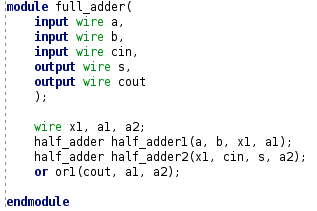
\includegraphics[width=0.5\textwidth]{Full Adder Code.png}
        \caption{Full Adder Code}
        \label{fig:Full-Adder-Code}
    \end{figure}
    \par Shown above is the code for the implementation of the full adder with
    the use of the Verilog HDL. In this case, the inputs are given as $a$, $b$,
    and $cin$, while the outputs are given as $s$ and $cout$. Here, the sum that
    is outputted is the full sum of the two inputs. The logic used in this case
    actually utilizes the previous module that was defined named "half\_adder."
    In this case, the implementation relies on the iteration of the user defined
    function in addition with the "or" function which is used to define the OR
    gate that outputs the full carry out of the system. The term "wire" is used
    to define wires used to connect the first half adder to the second, as well
    as the outputs of the full adder to the input of the OR gate.
    \section*{Four-Bit Adder/Subtractor}
    \begin{figure}[h]
        \centering
        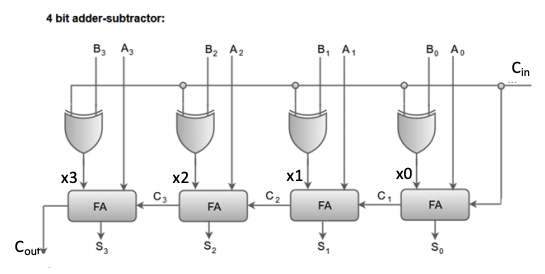
\includegraphics[width=0.8\textwidth]{4-bit Adder-Subtractor Design.png}
    \end{figure}
    \par This this the general design for the four bit adder/subtractor and it
    can be seen that it is exclusively contracted of full adders and XOR gates.
    The main attribute to note here about the adder is that one of its inputs is
    not direct rather, it is the output of an XOR gate. Isolating one adder, we
    can see that the two inputs, usually $A$ and $B$, are taken as $A_0$ and
    $B_0 \oplus C_{in}$. The reason for this is due to the fact that this is a
    dual functioning device, responsible for summation as well as subtraction.
    By utilizing an XOR gate to control one of the inputs, the input will be
    changed based on the value of $C_{in}$, and with that will come the change
    to the function of the device. If the carry in is set to 0, the 4-bit input
    will be added and if $C_{in}$ is set to 1, the device will subtract the
    input numbers. This is more evident when the truth table for one adder in
    this design is analyzed.
    \begin{table}[h]
        \centering
        \begin{tabular}{cccc|cc}
            \toprule
            $C_{in}$ & $A_0$ & $B_0$ & $B_0 \oplus C_{in}$ & $S_0$ & $C_{out}$ \\
            \midrule
            0 & 0 & 0 & 0 & 0 & 0 \\
            0 & 0 & 1 & 1 & 1 & 0 \\
            0 & 1 & 0 & 0 & 1 & 0 \\
            0 & 1 & 1 & 1 & 0 & 1 \\
            1 & 0 & 0 & 1 & 0 & 1 \\
            1 & 0 & 1 & 0 & 1 & 0 \\
            1 & 1 & 0 & 1 & 1 & 1 \\
            1 & 1 & 1 & 0 & 0 & 1 \\
            \bottomrule
        \end{tabular}
    \end{table}
    \par This is the logic table for the first bit in the input sequence. Here,
    the values of $A_0$ and $B_0$ are being compared, and based on the value of
    $C_{in}$ the bits are either added or subtracted. The reason this provides
    functional operation is due to the inherent function of the XOR gate. The
    expression of an XOR gate with the inputs $X$ and $Y$ can be written as,
    $X'Y+XY'$. With this, if we set $Y$ equal to 1, it can be seen that the
    output of the gate will be $X'$. The opposite is true if $Y$ equals 0, the
    output will be $X$.  Using this, since the inputs of the XOR gate are
    $C_{in}$ along with one of the input bits, the input bit that is being
    varied switches from $B$, when $C_{in}$ is 0, to $B'$, when $C_{in}$ equals
    1. In this case, $B$ is the bit $B_0$ and with the fluctuation of $C_{in}$
    from 0 to 1, the output of the adder, $S_0$, will either be the sum of $B_0$
    and $A_0$ or, their difference.  The same function is attributed to the
    other input bits and in the end what is resulted from device as a whole, is
    the full sum or difference of the 4-bit input numbers.
    \begin{figure}[h]
        \begin{minipage}{.5\textwidth}
            \centering
            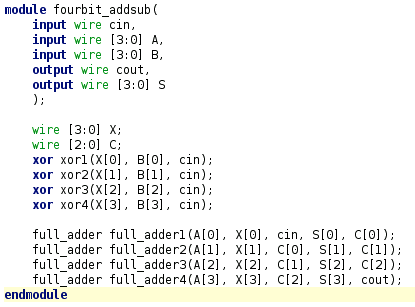
\includegraphics[width=0.9\textwidth]{Indexed AddSub Code.png}
        \end{minipage}
        \begin{minipage}{.55\textwidth}
            \centering
            \includegraphics[width=1.0\textwidth]{Indexed 4-bit Adder-Subtractor
            Schematic.png}
        \end{minipage}
        \caption{Code and Schematic for Adder/Subtractor}
    \end{figure}
    \newpage
    \par Above is the code and the generated schematic for the adder/subtractor
    as written using indexed input variables. This is done to make the code more
    readable and lessen the amount which has to be written as well as keeping
    the inputs and outputs organized within their respective domains. Here, the
    inputs are defined as, $cin$, $A_0-A_3$, and $B_0-B_3$. The indexing allows
    the user to write the terms for $A_0-A_3$ simply as $[3:0]\ A$, where the
    bracketed portion specifies the range and the latter half give the variable
    a name. This is much more efficient that writing individually, $a_0$, $a_1$,
    $a_2$, and $a_3$, and allows the variables to be accessed by accessing an
    index within the array rather than specifically calling each one
    individually. The outputs generated will be the carry out, $cout$, as well
    as the three individual sum or difference terms that are outputted from the
    full adders. The logic for this circuit requires the "xor" function as well
    as the instantiation of "fuller\_adder" module that was defined previously.
    \par In the code the wires $X$ and $C$ are defined and are used in the
    connection of the adder modules to one another. The three defined $X$ wires
    are formed as the outputs of the XOR gates that are connected to the $B$
    input bit and $C_{in}$, and the $C$ wire is used for sending the carry out
    of one adder as the carry in of the next adder. Next, the XOR gates are
    formed and they take the individual bits of the input $B$ as well as
    $C_{in}$ and output to one of the wires, $X$. Then the full adders are
    instantiated and they are responsible for the formation of the sum terms as
    well as the carry outs. The first three adders are interconnected and take
    the values of the input bit $A$ and the wires carrying the output of the XOR
    gates, $X$, and output one of the wires, $C$, as the individual carry outs
    which are taken as the carry ins of the next adder. The final adder outputs
    a sum term and the variable $cout$, the final carry out. The process of
    these incremental changes can be seen by creating a simulation of the device
    where all nine inputs are present. With the analysis of the waveform
    generated by this simulation, how exactly these changes occur can be
    visualized.
    \begin{figure}[h]
        \centering
        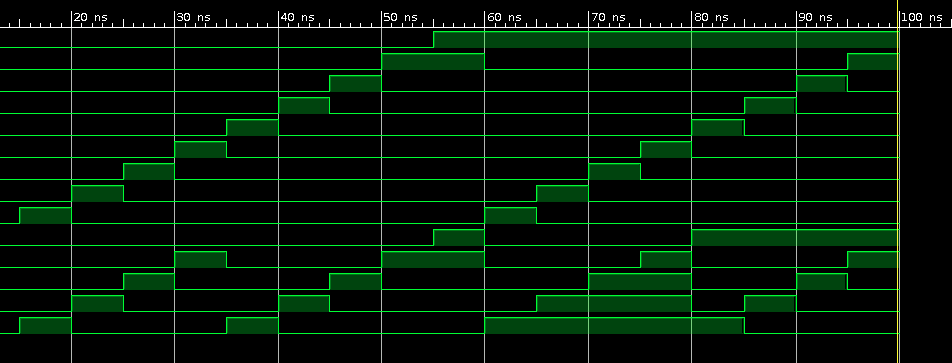
\includegraphics[width=0.8\textwidth]{Waveform.png}
        \caption{Waveform for Adder/Subtractor}
        \label{fig:Waveform}
    \end{figure}
    \par This is the waveform generated for the adder and subtractor module and
    all nine inputs can be seen here as they change in value. Starting from the
    top wave, this is the input $Cin$ since it can be seen to change from 0 to 1
    only once, in the middle of the diagram. The rest of the inputs going down
    are $a_0-a_3$ and then $b_0-b_3$, $cout$, and finally the three sum terms,
    $s_0-s_3$. The code for this can also be analyzed to see how this simulation
    was put together and will give insight about how the function of such a
    device is achieved.
    \begin{figure}[h]
        \centering
        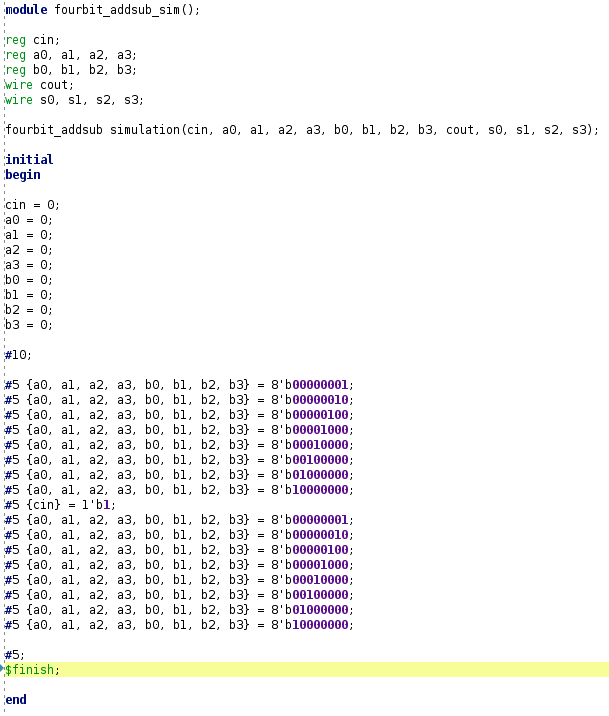
\includegraphics[width=0.6\textwidth]{Simulation Code.png}
        \caption{Simulation Code}
        \label{fig:Simulation-Code}
    \end{figure}
    \par Here, the code is shown as it simulates the behavior of the nine input
    adder and subtractor. The first step to setting up a simulation is to
    initialize the inputs and outputs. The "reg" statement is used to achieve
    this and the outputs are simply defined as wires as they are not independent
    variables. Next, the simulation is given a name, "fourbit\_addsub", and the
    inputs and outputs are specified as arguments to the built-in "simulation"
    function. Now, the setup is complete and the parameters for the simulation
    can be defined.
    \par With the "initial" statement, we dictate the start to the simulation.
    The individual inputs are then all given starting values, in this case
    000000000 for all the inputs. The actual waveform data is produced by the
    changes in the inputs and how these changes effect the output so, the inputs
    must be changed systematically in order to monitor the changes in the
    outputs. The last function that is called is the "finish" function at the
    end. This specifies the end of the simulation and thus the conclusion of the
    waveform.
\end{document}
